\documentclass[a4paper,12pt]{article}
\usepackage{../../mypackages}
\usepackage{../../macros}

\setlength{\parindent}{0pt}

\begin{document}

\title{Chapitre 4 : L'atome / Les molécules}
\author{N. Bancel}
\date{Octobre 2024}

\maketitle

\section{Exercice 1}

\begin{figure}[H]
  \centering
  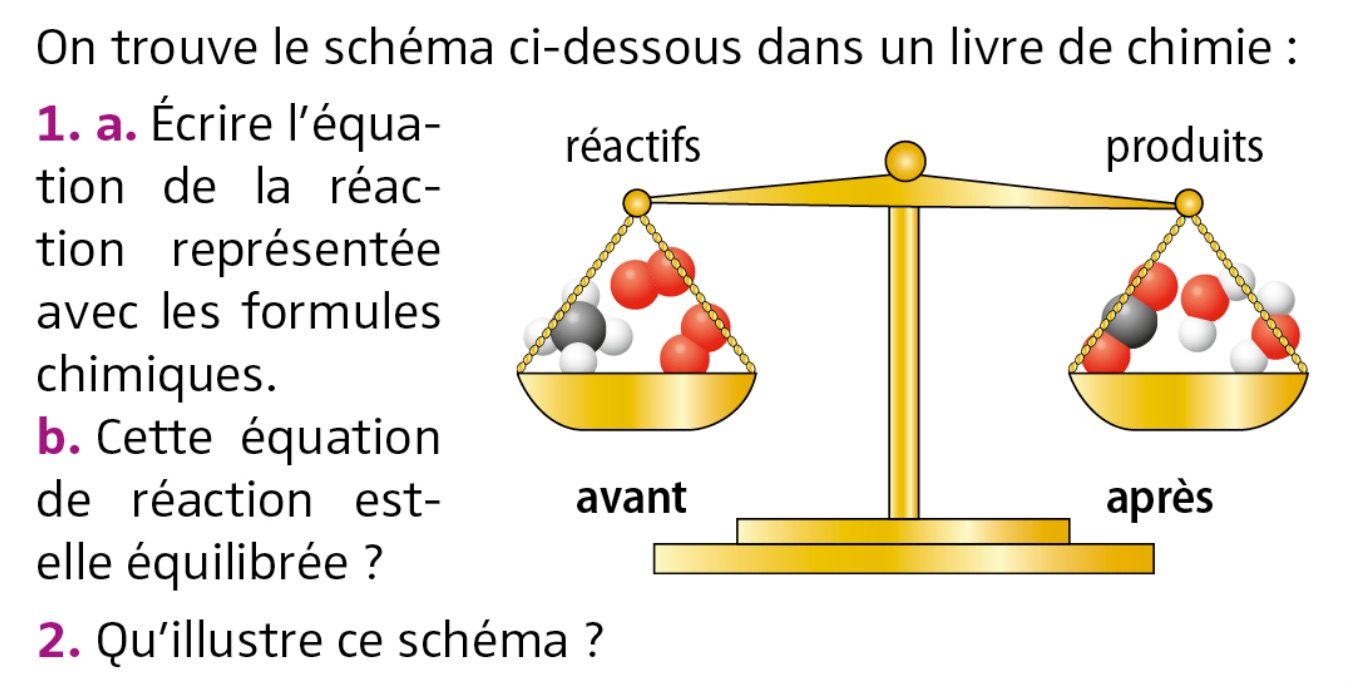
\includegraphics[width=0.8\linewidth]{04_02_01.jpg}
  \caption{Exercice 1}
\end{figure}

\begin{enumerate}[label=\textbf{1.\alph*}]
    \item \textbf{Écriture de l'équation de la réaction chimique}\\
    En observant les molécules présentes dans les plateaux de la balance, on reconnaît la réaction suivante :
    \[
    \ce{CH4 + 2 O2 -> CO2 + 2 H2O}
    \]
    où \ce{CH4} représente le méthane, \ce{O2} le dioxygène, \ce{CO2} le dioxyde de carbone, et \ce{H2O} l'eau.

    \begin{tcolorbox}[colback=blue!10!white, colframe=blue!75!black, title=Attention]
      Attention à ne pas confondre : ce n'est pas parce qu'on voit qu'il y a 4 atomes d'oxygène dans les réactifs qu'il faut se dire que \ce{O4} est un réactif. \\
      Cette molécule n'existe pas. \\
      On observe 2 molécules distinctes, composées de 2 atomes d'oxygène chacune : c'est donc \ce{2 O2} dans la formule (2 molécules de dioxygène)
    \end{tcolorbox}

    \item \textbf{Vérification de l'équilibrage de l'équation}\\
    Comptons les atomes de chaque élément de part et d'autre de l'équation :
    \begin{itemize}[noitemsep]
        \item Atomes de carbone (C) : 1 à gauche (côté "réactifs"), 1 à droite (côté "réactifs")
        \item Atomes d'oxygène (O) : 4 à gauche, 4 à droite (2 venant de \ce{2 H2O}, 2 venant de \ce{CO2})
        \item Atomes d'hydrogène (H) : 4 à gauche, 4 à droite
    \end{itemize}
    Il y a le même nombre d'atomes du même type du côté des réactifs que du côté des produits : l'équation est donc bien équilibrée. On pouvait s'y attendre : l'équation est équilibrée (on a compté exactement le même nombre d'atomes du même type du côté des réactifs et du côté des produits, donc la masse des réactifs = la masse des produits)

\end{enumerate}

\noindent
\textbf{2. Ce que représente le schéma :} \\
Le schéma illustre la conservation de la masse lors d'une réaction chimique, c'est-à-dire que la masse des réactifs est égale à la masse des produits, conformément à la loi de Lavoisier.

\section{Exercice 2}

\begin{figure}[H]
  \centering
  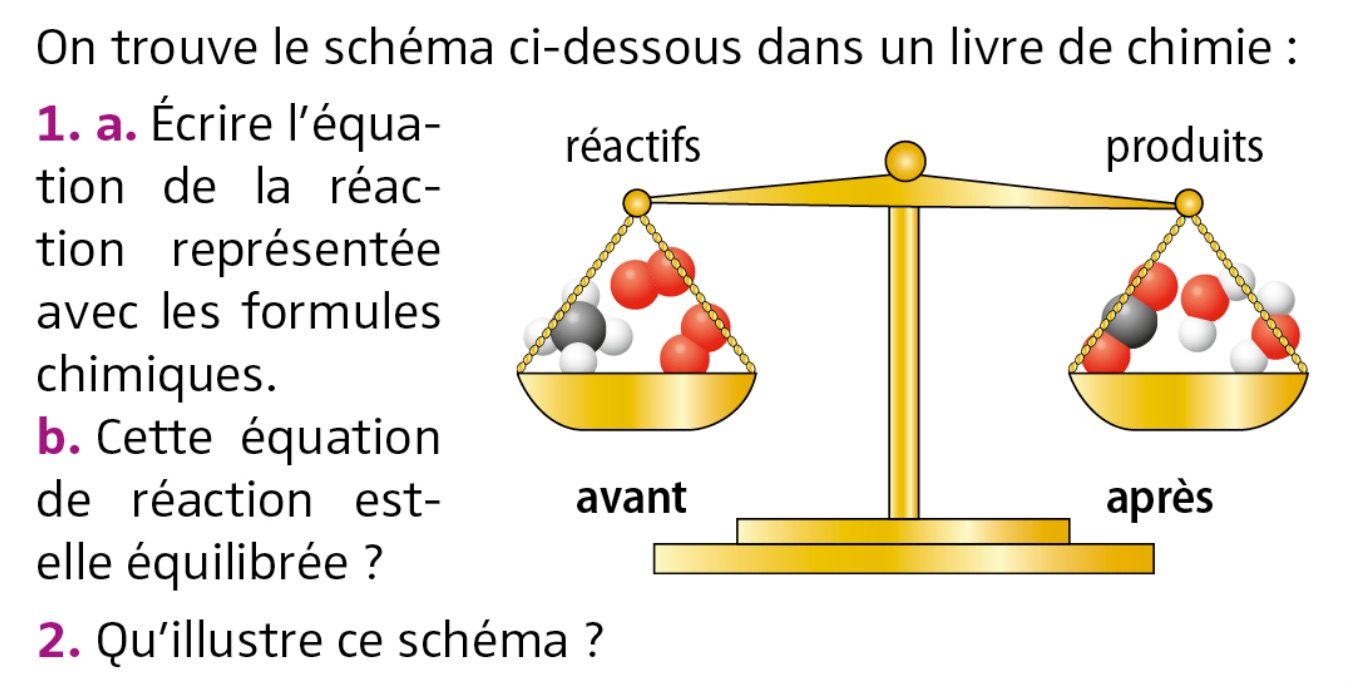
\includegraphics[width=0.8\linewidth]{04_02_01.jpg}
  \caption{Exercice 2}
\end{figure}

\begin{enumerate}[label=\textbf{\arabic*.}]
    \item \textbf{Équation de réaction en toutes lettres}\\
    Lorsqu'on mélange de l'alcool isoamylique (ai) et de l'acide éthanoïque (ae), on obtient de l'arôme de banane et de l'eau. La réaction est :
    \[
    \text{alcool isoamylique} + \text{acide éthanoïque} \rightarrow \text{arôme de banane} + \text{eau}
    \]

    \item \textbf{Calcul de la masse après la transformation chimique}\\
    
    \textcolor{orange}{\textbf{Raisonnement}}

    On appelle $m_{ai}$ la masse d'alcool isoamylique \\
    On appelle $m_{ae}$ la masse d'acide éthanoïque \\
    La masse totale des réactifs est notée $m_{totale\_reactifs}$ \\

    On peut écrire que 
    
    \[
    m_{totale\_reactifs} = m_{ai} + m_{ae}
    \]

    En appliquant les formules de la masse volumique, on sait que, avec
    \begin{itemize}[noitemsep]
      \item $V_{ai}$ : Volume d'alcool isoamylique
      \item $\rho_{ai}$ : masse volumique de l'alcool isoamylique
      \item $V_{ae}$ : Volume d'acide éthanoïque
      \item $\rho_{ae}$ : masse volumique de l'acide éthanoïque
    \end{itemize}
    
    \begin{align*}
      m_{ai} &= V_{ai} \times \rho_{ai} \\
      m_{ae} &= V_{ae} \times \rho_{ae} \\
      \intertext{donc} \\
      m_{totale\_reactifs} &= V_{ai} \times \rho_{ai} + V_{ae} \times \rho_{ae}
    \end{align*}
    
    \textcolor{orange}{\textbf{Application numérique}}

    Données :
    \begin{itemize}
        \item Volume d'alcool isoamylique $V_{ai} = 10$ mL et masse volumique $\rho_{ai} = 0.81$ g/mL
        \item Volume d'acide éthanoïque $V_{ae} = 10$ mL et masse volumique $\rho_{ae} = 1.05$ g/mL
    \end{itemize}

    Calcul des masses :
    \[
    m_{ai} = V_{ai} \times \rho_{ai} = 10 \times 0.81 = 8.1 \, \text{g}
    \]
    \[
    m_{ae} = V_{ae} \times \rho_{ae} = 10 \times 1.05 = 10.5 \, \text{g}
    \]
    \[
    m_{totale\_reactifs} = m_{ai} + m_{ae} = 8.1 + 10.5 = 18.6 \, \text{g}
    \]
  
  \textcolor{orange}{\textbf{Conclusion / Interprétation}} \\
  On vient de calculer la masse des réactifs, \textbf{pas celle des produits}. Mais selon la loi de conservation de la masse, on sait que ces deux masses sont égales, donc la masse totale des produits sera également de 18,6 g.

\end{enumerate}

\section{Exercice 3}

Dans chaque réaction ci-dessous, identifions les réactifs et produits, et équilibrons les équations.


\begin{enumerate}
  \item \textbf{Réaction de combustion du propane}

  Équation non équilibrée :
  \[
  \ce{C3H8 + O2 -> CO2 + H2O}
  \]

  Explications :
  \begin{itemize}
      \item Le propane (\ce{C3H8}) réagit avec le dioxygène (\ce{O2}) pour former du dioxyde de carbone (\ce{CO2}) et de l'eau (\ce{H2O}).
      \item Pour équilibrer cette équation, commençons par les atomes de carbone : il y a 3 atomes de carbone dans \ce{C3H8}, donc nous devons mettre un coefficient 3 devant \ce{CO2} pour avoir 3 atomes de carbone du côté des produits.
      \item Ensuite, équilibrons les atomes d'hydrogène : \ce{C3H8} contient 8 atomes d'hydrogène, donc nous mettons un coefficient 4 devant \ce{H2O} pour obtenir 8 atomes d'hydrogène du côté des produits.
      \item Finalement, équilibrons les atomes d'oxygène : il y a maintenant 10 atomes d'oxygène du côté des produits (3 molécules de \ce{CO2} contiennent 6 atomes d'oxygène et 4 molécules de \ce{H2O} contiennent 4 atomes d'oxygène), donc nous mettons un coefficient 5 devant \ce{O2} du côté des réactifs.
  \end{itemize}
  Équation équilibrée :
  \[
  \ce{C3H8 + 5 O2 -> 3 CO2 + 4 H2O}
  \]

  \item \textbf{Formation du peroxyde d'hydrogène}

  Équation non équilibrée :
  \[
  \ce{H2O + O2 -> H2O2}
  \]

  Explications :
  \begin{itemize}
      \item Ici, l'eau (\ce{H2O}) réagit avec le dioxygène (\ce{O2}) pour produire du peroxyde d'hydrogène (\ce{H2O2}).
      \item Pour équilibrer, nous voyons qu'il y a 2 atomes d'oxygène dans \ce{O2} mais un seul dans chaque molécule de \ce{H2O2}. Nous ajoutons donc un coefficient 2 devant \ce{H2O} et \ce{H2O2} pour équilibrer les atomes d'oxygène.
  \end{itemize}
  Équation équilibrée :
  \[
  \ce{2 H2O + O2 -> 2 H2O2}
  \]

  \item \textbf{Combustion du méthane}

  Équation non équilibrée :
  \[
  \ce{CH4 + O2 -> CO2 + H2O}
  \]

  Explications :
  \begin{itemize}
      \item Le méthane (\ce{CH4}) réagit avec le dioxygène (\ce{O2}) pour produire du dioxyde de carbone (\ce{CO2}) et de l'eau (\ce{H2O}).
      \item D'abord, équilibrons les atomes de carbone en mettant un coefficient 1 devant \ce{CO2}.
      \item Ensuite, équilibrons les atomes d'hydrogène en ajoutant un coefficient 2 devant \ce{H2O}.
      \item Enfin, équilibrons les atomes d'oxygène en ajoutant un coefficient 2 devant \ce{O2}.
  \end{itemize}
  Équation équilibrée :
  \[
  \ce{CH4 + 2 O2 -> CO2 + 2 H2O}
  \]

  \item \textbf{Décomposition de l'eau}

  Équation non équilibrée :
  \[
  \ce{H2O -> H2 + O2}
  \]

  Explications :
  \begin{itemize}
      \item L'eau (\ce{H2O}) se décompose en dihydrogène (\ce{H2}) et dioxygène (\ce{O2}).
      \item Pour équilibrer les atomes d'hydrogène, mettons un coefficient 2 devant \ce{H2O}.
      \item Il y a maintenant 2 atomes d'oxygène des deux côtés de l'équation.
  \end{itemize}
  Équation équilibrée :
  \[
  \ce{2 H2O -> 2 H2 + O2}
  \]

  \item \textbf{Synthèse de l'ammoniac}

  Équation non équilibrée :
  \[
  \ce{N2 + H2 -> NH3}
  \]

  Explications :
  \begin{itemize}
      \item L'azote (\ce{N2}) réagit avec l'hydrogène (\ce{H2}) pour former de l'ammoniac (\ce{NH3}).
      \item Nous équilibrons les atomes d'azote en ajoutant un coefficient 2 devant \ce{NH3}.
      \item Ensuite, équilibrons les atomes d'hydrogène en ajoutant un coefficient 3 devant \ce{H2}.
  \end{itemize}
  Équation équilibrée :
  \[
  \ce{N2 + 3 H2 -> 2 NH3}
  \]

  \item \textbf{Combustion de l'éthane}

  Équation non équilibrée :
  \[
  \ce{C2H6 + O2 -> CO2 + H2O}
  \]

  Explications :
  \begin{itemize}
      \item L'éthane (\ce{C2H6}) réagit avec le dioxygène (\ce{O2}) pour produire du dioxyde de carbone (\ce{CO2}) et de l'eau (\ce{H2O}).
      \item Équilibrons les atomes de carbone en ajoutant un coefficient 2 devant \ce{CO2}.
      \item Ensuite, équilibrons les atomes d'hydrogène en ajoutant un coefficient 3 devant \ce{H2O}.
      \item Pour finir, mettons un coefficient 7 devant \ce{O2}.
  \end{itemize}
  Équation équilibrée :
  \[
  \ce{2 C2H6 + 7 O2 -> 4 CO2 + 6 H2O}
  \]

  \item \textbf{Formation de monoxyde de carbone}

  Équation non équilibrée :
  \[
  \ce{C + O2 -> CO}
  \]

  Explications :
  \begin{itemize}
      \item Le carbone réagit avec le dioxygène pour former du monoxyde de carbone (\ce{CO}).
      \item Pour équilibrer l'oxygène, mettons un coefficient 2 devant \ce{CO}.
  \end{itemize}
  Équation équilibrée :
  \[
  \ce{2 C + O2 -> 2 CO}
  \]

  \item \textbf{Combustion de l'alcool méthylique}

  Équation non équilibrée :
  \[
  \ce{CH4O + O2 -> CO2 + H2O}
  \]

  Explications :
  \begin{itemize}
      \item L'alcool méthylique (\ce{CH4O}) réagit avec le dioxygène pour produire du dioxyde de carbone et de l'eau.
      \item Équilibrons les atomes de carbone et d'hydrogène en ajustant les coefficients.
  \end{itemize}
  Équation équilibrée :
  \[
  \ce{CH4O + O2 -> CO2 + 2 H2O}
  \]

\end{enumerate}
\section{Exercice 4}

\begin{figure}[H]
  \centering
  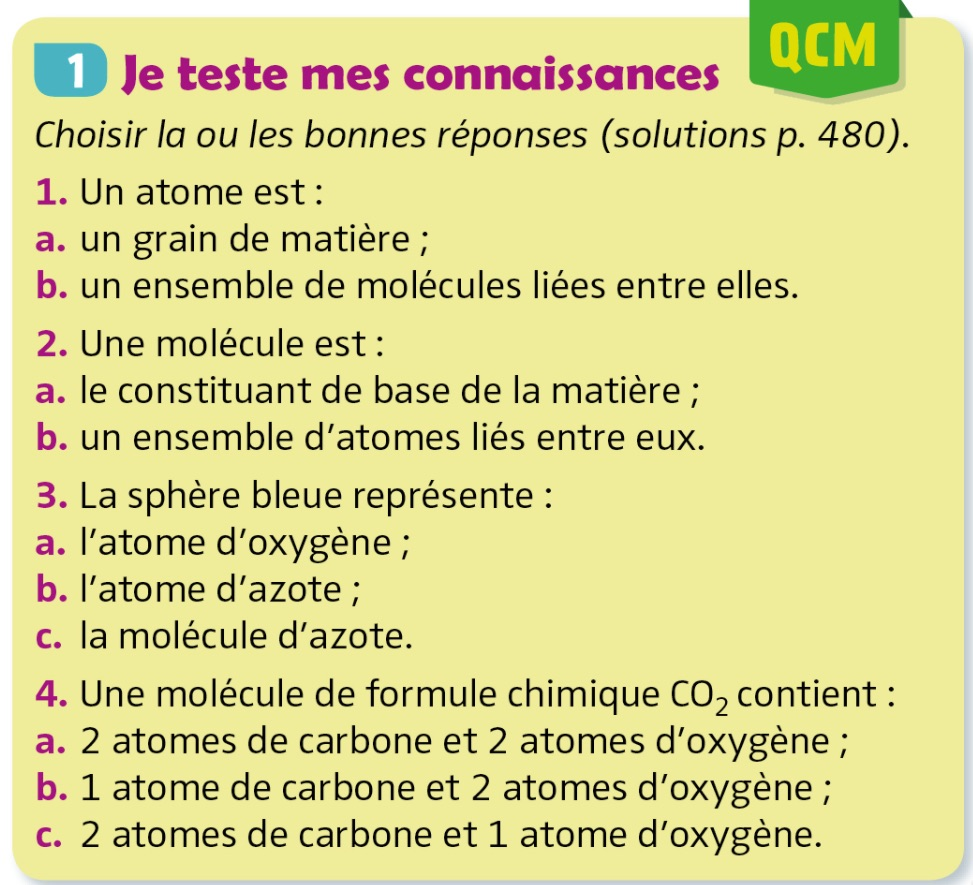
\includegraphics[width=0.9\linewidth]{04_02_03.jpg}
  \caption{\label{} Exercice 1}
\end{figure}

\textbf{Correction :}

\begin{enumerate}
    \item \textbf{Un atome est :} \newline
    \textbf{Réponse :} a. un grain de matière. \newline
    \textit{Justification :} Un atome est la plus petite unité constitutive de la matière. Il est composé d'un noyau entouré d'électrons et représente la base des éléments chimiques.

    \item \textbf{Une molécule est :} \newline
    \textbf{Réponse :} b. un ensemble d'atomes liés entre eux. \newline
    \textit{Justification :} Une molécule est formée par la liaison chimique d'au moins deux atomes. Ces atomes peuvent être identiques (comme dans \ce{O2}) ou différents (comme dans \ce{H2O}).

    \item \textbf{La sphère bleue représente :} \newline
    \textbf{Réponse :} a. l'atome d'oxygène. \newline
    \textit{Justification :} Dans de nombreux schémas de modélisation moléculaire, les atomes d'oxygène sont souvent représentés par des sphères bleues pour les distinguer des autres types d'atomes.

    \item \textbf{Une molécule de formule chimique CO$_2$ contient :} \newline
    \textbf{Réponse :} b. 1 atome de carbone et 2 atomes d'oxygène. \newline
    \textit{Justification :} La formule chimique CO$_2$ indique qu'une molécule de dioxyde de carbone est composée d'un atome de carbone (C) et de deux atomes d'oxygène (O).
\end{enumerate}

\section{Exercice 5}

\begin{figure}[H]
  \centering
  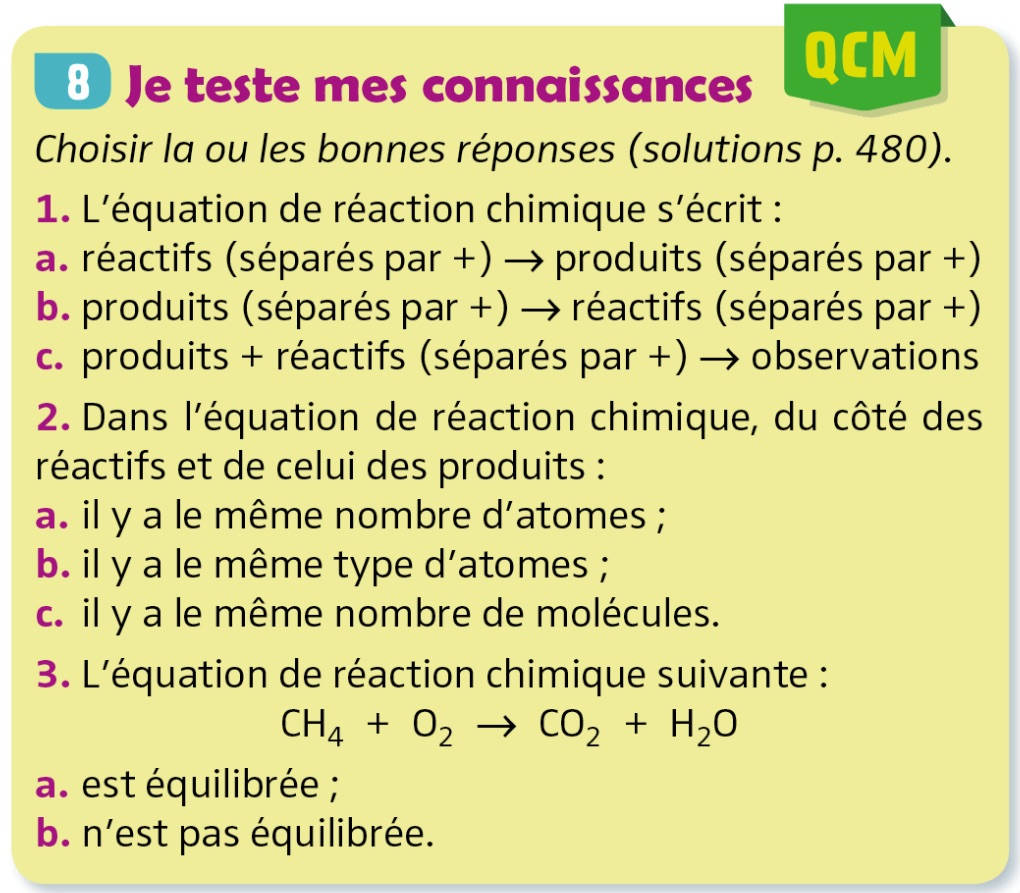
\includegraphics[width=0.9\linewidth]{04_02_04.jpg}
  \caption{\label{} Exercice 2}
\end{figure}

\textbf{Correction :}

\begin{enumerate}
    \item \textbf{L'equation de reaction chimique s'ecrit :} \\
    \textbf{Réponse :} a. Réactifs (separes par +) $\rightarrow$ produits (separes par +). \\
    \textit{Justification :} Une équation chimique décrit le processus de transformation des réactifs en produits. Les réactifs sont toujours placés à gauche de la flèche et les produits à droite.

    \item \textbf{Dans l'\'equation de r\'eaction chimique, du c\^ot\'e des r\'eactifs et de celui des produits :} \newline
    \textbf{Réponse :} a. il y a le m\^eme nombre d'atomes. \newline
    \textit{Justification :} La loi de conservation de la masse stipule que le nombre d'atomes de chaque élément doit être le même des deux côtés de l'équation chimique. Cela garantit que la matière n'est ni créée ni détruite.

    \item \textbf{L'equation de reaction chimique suivante : $\ce{CH4 + O2 -> CO2 + H2O}$} \newline
    \textbf{Réponse :} b. n'est pas equilibree. \newline
    \textit{Justification :} Comptons le nombre d'atomes de chaque côté :
    \begin{itemize}
        \item \textbf{Côté réactifs :} 1 atome de carbone (C), 4 atomes d'hydrogène (H) et 2 atomes d'oxygène (O) par molécule de O$_2$ (donc 2 $\times$ 1 = 2).
        \item \textbf{Côté produits :} 1 atome de carbone (C) dans CO$_2$, 2 atomes d'oxygène (O) dans CO$_2$ et 2 atomes d'hydrogène (H) et 1 atome d'oxygène (O) dans H$_2$O.
    \end{itemize}
    \textbf{Analyse :} On constate que le côté des réactifs contient 2 atomes d'oxygène, alors que le côté des produits en contient 3 (2 dans CO$_2$ + 1 dans H$_2$O). L'hydrogène est équilibré, mais l'oxygène ne l'est pas, prouvant ainsi que l'équation n'est pas équilibrée
\end{enumerate}

\section{Exercice 6}

\begin{figure}[H]
  \centering
  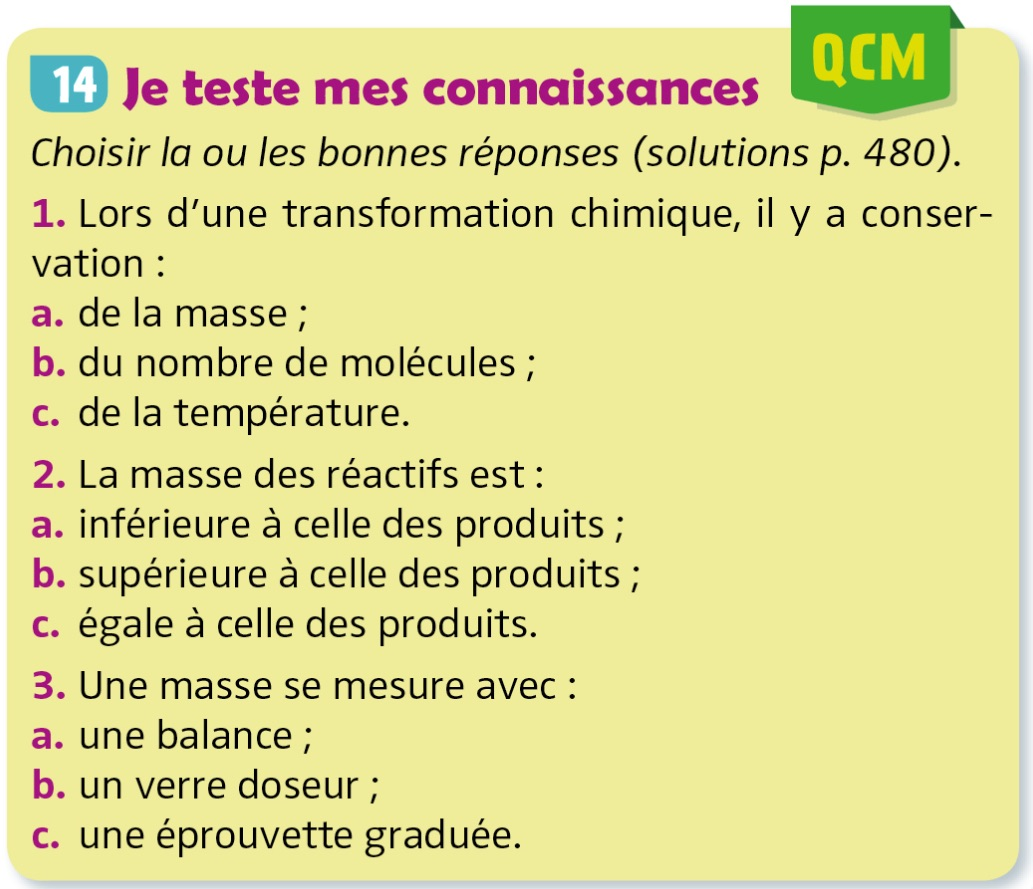
\includegraphics[width=0.9\linewidth]{04_02_05.jpg}
  \caption{\label{} Exercice 3}
\end{figure}

\textbf{Correction :}

\begin{enumerate}
    \item \textbf{Lors d'une transformation chimique, il y a conservation :} \newline
    \textbf{Réponse :} a. de la masse. \newline
    \textit{Justification :} Selon la loi de Lavoisier, la masse totale des réactifs est égale à la masse totale des produits dans une réaction chimique. La masse est donc conservée.

    \item \textbf{La masse des r\'eactifs est :} \newline
    \textbf{Réponse :} c. \`egale \`a celle des produits. \newline
    \textit{Justification :} En raison de la conservation de la masse lors d'une réaction chimique, la masse des réactifs doit toujours être égale à la masse des produits.

    \item \textbf{Une masse se mesure avec :} \newline
    \textbf{Réponse :} a. une balance. \newline
    \textit{Justification :} La balance est l'instrument utilisé pour mesurer la masse des substances. Les autres outils, comme le verre doseur ou l'éprouvette graduée, servent à mesurer des volumes.
\end{enumerate}

\end{document}
